\chapter{Pruning} \label{chapter3}


 \section{Introduction}
\label{sec:chap3-introduction}

Pruning is a very popular practice to decrease the cost and time of combining multiple detectors. There are mostly two important challenges when it comes to pruning. The first one is to determine where pruning should be applied (e.g., feature level, model level, etc.). The second challenge is to determine the pruning criteria.

Generally speaking, pruning can be done at four different levels: sensor level, feature level, matching score level, and decision level \cite{Tao2009}, as illustrated in Figure~\ref{fig::level_of_pruning}

 In this thesis, the main focus of pruning detectors is at the decision level. However, there are some scenarios that require pruning at the matching score level. When there are thousands of detectors, it does not make sense to convert them to a few response vectors and combine everything together, because  we will have too many redundant response vectors, which hinders the efficiency of the pruning process.


\begin{figure}[]
\centering
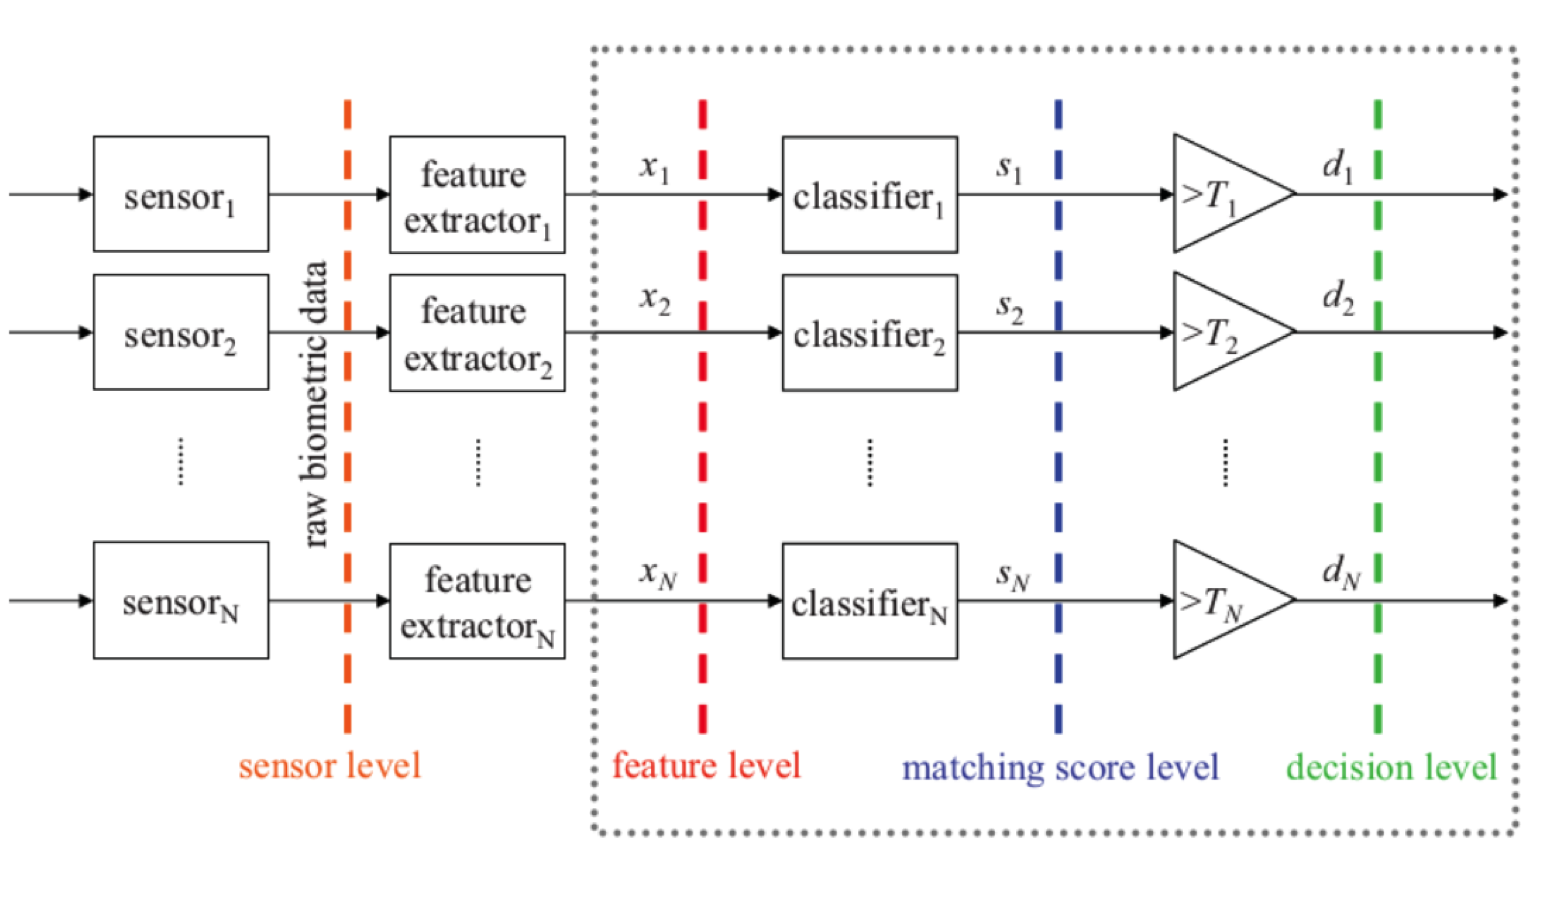
\includegraphics[width=1\linewidth]{figs/level-of-pruning}
\caption{Different levels of combination or pruning: sensor level, feature level, matching score level, and decision level \cite{Tao2009}.}
\label{fig::level_of_pruning}
\end{figure}

After seeing the different levels where pruning can be applied, the question is how to prune the pool of available detectors and make a basket of reasonable detectors. To have a reasonable basket of remaining detectors, two criteria should be considered.  

Firstly, there should be some accurate detectors in the basket, with this we guarantee that the minimum accuracy we obtain after pruning and the combination is not worse than any of the detectors we had in the pool. Also, by choosing and combining the accurate ones, we increase the chances of getting better results than combining two random or naïve detectors.  

Secondly, we need to be sure that we have a diverse basket of detectors. If very similar detectors  are selected  in the basket, we should not expect to see a major improvement after combining. Another thing that helps to increase the diversity of the basket is to try to find and select detectors that complement the errors of already selected detectors. Since we have already selected accurate detectors in the basket, it is a good practice to try to find the detectors that complement the errors these detectors exhibit. 

To see the importance of diversity and how it can help to improve the result of the combination, we show in the following example, importance of selecting the initial detectors and respective detectors compare to it, the one that tries to complement first detector's errors. And by combining these two detectors with a right Boolean operator with will reach a very promising result. As it is shown in Figure~\ref{fig::accurate_detector}, among all the trained detectors, we only one need to find a way to select a detector that is accurate,and in Figure~\ref{fig::diverse_detector}, we see that we are trying to select a detector, that is very diverse to previously selected one in order to increase the chance of getting better results after combination. The two selected detectors in Figure~\ref{fig::accurate_detector} and Figure~\ref{fig::diverse_detector} are completing each other error.


\begin{figure}[H]
\centering
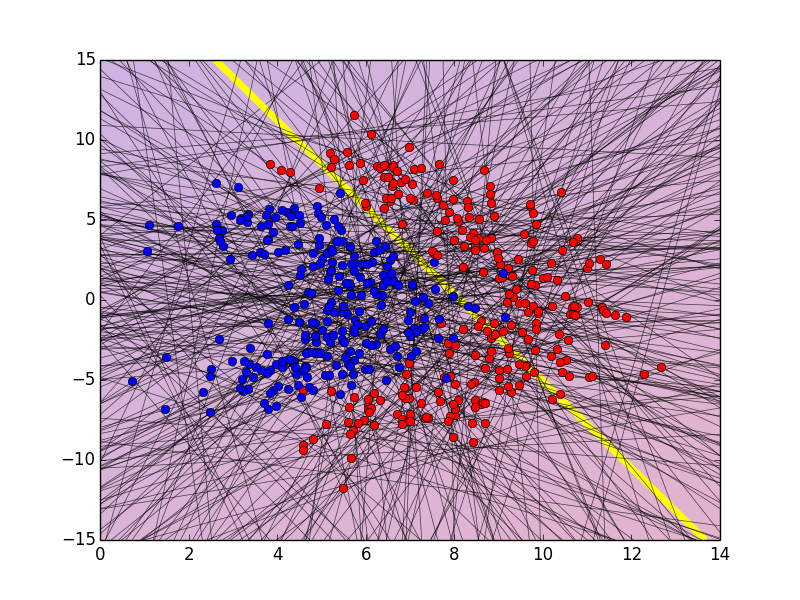
\includegraphics[width=1\linewidth]{figs/Lithuanian/Initial_detectors}
\caption{Selecting accurate detectors}
\label{fig::accurate_detector}
\end{figure}

\begin{figure}[H]
\centering
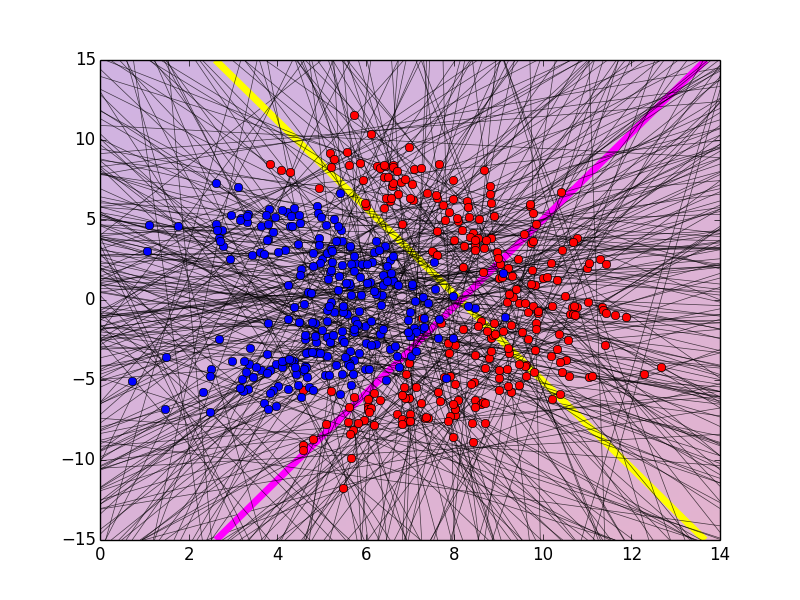
\includegraphics[width=1\linewidth]{figs/Lithuanian/complement_detectors}
\caption{Selecting diverse detector compares to previously selected}
\label{fig::diverse_detector}
\end{figure}


\section{Pruning Boolean Combination (PBC) Approach}
\label{sec:pbc}

In this section, we describe our Pruned Boolean Combination (PBC) algorithm, which is based on two novel pruning techniques that select a subset of diverse and accurate detectors for combination, while discarding the remaining ones, this happened at decision level.
PBC can avoid both the exponential explosion of combinations provided by the brute-force approach and the sequential combination of IBC.
The main difference is that the PBC algorithm proceeds by thresholding all available soft detectors into crisp ones.
This step is, in fact, not essential for PBC because thresholding could be done outside the algorithm and the crisp detectors are directly input for pruning.
In contrast with IBC, all available crisp detectors are input to one of the proposed pruning techniques, MinMax-Kappa or ROCCH-Kappa described in Section~\ref{sub:minmax-kappa}~and~\ref{sub:rocch-kappa}, to select the best subset of crisp detectors for Boolean combination and control its size $U$ (i.e., the number of combined detectors).
Without pruning brute-force pairwise combination of all available detectors may not be feasible for large number of detectors, $\mathcal{O}({N^2})$ (where N is number of available detectors), for further details see Section~\ref{sub:complexity}.
 
After seeing the main pruning idea in Section~\ref{sub:minmax-kappa}~and~\ref{sub:rocch-kappa} we introduce a different distance correlation (measure of agreement between vecotrs or dependence coefficient) ~\ref{sec:dcov-dcor} rather than kappa to show that the results of PBC are consistent, and as long as a proper measure is used we can get promising result either using it with MinMax- or ROCCH-. In Section~\ref{sub:minmax-rocch-dcov} we explained how we used the MinMax and ROCCH technique again and just changed the measure of agreement from kappa to Dcor or Dcov to prune the pool of detectors.

The boost in performance achieved with an ensemble of detectors is often attributed to the concept of diversity.
While it is generally accepted that an ensemble should contain diverse models to improve the performance, there is no clear definition of diversity neither a consensus about the measure of diversity and its computation.
In practice, several measures of diversity have been proposed to quantify the level of agreement or measure the dependency among the ensemble members \cite{Kuncheva2003b}.


%%%%%%%%%%%%%%%%%%%%%%%%%%%%%%%%%%
\subsection{Kappa Measure}
\label{sec:kappa}

Cohen's Kappa statistic (or simply Kappa hereafter) is one of the well-known and widely used measure of agreement between raters \cite{Cohen1995a}.
Kappa has lately gained some popularity for ensemble combination, especially the Kappa-error diagrams which help visualizing individual accuracy and diversity in a two dimensional plot \cite{Margineantu1997,Kunchev2013}.
Our pruning techniques, described in the next sections, are based on Kappa and inspired by the Kappa-error diagram only for visualization of Kappa against the false positives and true positives (as shown in Figures~\ref{fig:MinMax-Kappa-fpr-tpr}~and~\ref{fig:ROCCH-Kappa-fpr-tpr}).

\begin{table}[tbh]
    \normalsize
    \centering
    \renewcommand{\arraystretch}{1.3}
    \caption{Contingency table between two detector decisions}
    \label{Table::Contigency}
    \centering
    \begin{tabular}{ r|c|c| }
        \multicolumn{1}{r}{}
	 &  \multicolumn{1}{c}{$D_2$ correct}
	 & \multicolumn{1}{c}{$D_2$ wrong} \\
	\cline{2-3}
	$D_1$ correct & a & b \\
	\cline{2-3}
	$D_1$ wrong & c & d \\
	\cline{2-3}
    \end{tabular}
\end{table}

Consider the contingency table of two detectors, $D_1$ and $D_2$, presented in Table~\ref{Table::Contigency}, where, for instance, $a$ is the number of examples on which both detectors agree.
The sum of all element in Table~\ref{Table::Contigency} is equal to the size of validation set, $a+b+c+d=|\mathcal{V}|$.
The Kappa ($\kappa$) measure between two detectors is therefore computed based on the element of the contingency table according to Equation~\ref{eq:Kappa}.
\begin{equation}
  \kappa =  \cfrac{2(ad-bc)}{(a+b)(b+d) + (a+c)(c+d) }
  \label{eq:Kappa}
\end{equation}
Kappa takes on values between $-1$ and $1$; lower values means a high level of disagreement or more diverse opinions, while higher values indicate a high level of agreement or similarity in responses between detectors.
When both detectors provide the same vector of decisions (they agree on every example) then $\kappa=1$.
On the other hand, when $\kappa=0$ the detectors are independent (any agreement is totally due to chance).
Negative Kappa values can be interpreted as both detectors agrees less than what would be expected just by chance.
More importantly, negative values account for negative correlations, which can be useful for combination, but this rarely occurs in practice \cite{Margineantu1997}.  % which can


\subsection{Distance Covariance (dcov) and Distance Correlation  (dcor) Measure}
\label{sec:dcov-dcor}
Distance correlation is a measure of statistical dependence between two vectors of arbitrary. The measure of dependence is zero if and only if the random variables are statistically independent. Distance correlation is a new measure of dependence between random vectors introduced by~\cite{Szekely2009}.

In order to understand the definition of distance covariance and distance correlation we should first start with distance covariance.

Assume we have two random vecors, the vecotrs are $X_n$ and $Y_n$, $k=1,2,...,n$. Fristly we should compute all piarwise distances:

$a_{j,k} = ||X_j - X_k||$

$b_{j,k} = ||Y_j - Y_k||$

By this, we computed the n by n distance matrices (aj, k) and (bj, k). After this we need to calculate all doubly centered distances:

\begin{equation}
\label{eq:doubly_a}
A_{j,k} := a_{j,k} - \bar{a}_{j.} - \bar{a}_{.k} + \bar{a}_{..}
\end{equation}

\begin{equation}
\label{eq:doubly_b}
B_{j,k} := b_{j,k} - \bar{b}_{j.} - \bar{b}_{.k} + \bar{b}_{..}
\end{equation}

In equation~\ref{eq:doubly_a} $\bar{a}_{j.}$ is the j-th row mean, $\bar{a}_{.k}$ is the k-th column mean, and $\bar{a}_{..}$ is the grand mean of the distance matrix of the X sample. The exact same notation applies on $b$ too. One thing to note is that in the matrices of centered distances $A_{j, k}$ and $B_{j,k}$  sum of all rows and all columns equal to zero.

By having all of these value we can calculate the distance covariance like this:

\begin{equation}
\label{eq:distance_covariance}
dCov_n^2 (X, Y) := \frac{1}{n^2} \sum_{j,k=1}^{n} A_{j,k}B_{j,k}
\end{equation}

Interesting point about distance coveriance is that we can define it with help of Pearson’s covariance.




\begin{equation}
\label{eq:distance_covariance_peasron}
dCov^2 (X, Y) := cov(|| X - X^{\prime}||, || Y - Y^{\prime}||) -  2cov(|| X - X^{\prime}||, || Y - Y^{\prime\prime}||)
\end{equation}

After calculating the distance covariance we can use it to calculate distance correlation, The distance correlation of two random vectors is calculated by dividing their distance covariance by the product of their distance standard deviations. 

\begin{equation}
\label{eq:distance_correlation}
dCor (X, Y) := \frac{dCov(X,Y)}{\sqrt{dVar(X)dVar(Y)}}
\end{equation}

%%%%%%%%%%%%%%%%%%%%%%%%%%%%%%%%%%
\subsection{MinMax-Kappa Pruning}
\label{sub:minmax-kappa}

% Keep this: Idea: we can not rely on absolute values for dependency /independence
% Some suggested upper and lower values on kappa (0.8) for dependent and independent
% However, there is no agreement.
% In our experiment

The proposed pruning technique starts by computing the Kappa values between each detector's decision vector and the true decision labels (or ground truth), and then sorting them in ascending order.
Detectors with large Kappa values ($\kappa \approx \kappa_{max}$) are accurate and hence should be selected; however, they provide less diverse decisions among themselves.
Therefore, the technique attempts to select complementary detectors by choosing those with Kappa values close to $\kappa \approx \kappa_{min}$.
In practice, $\kappa_{max}$ and $\kappa_{min}$ values depend on the data and the detectors.
Trivial detectors (providing always either positive or negative decisions) also reside at $\kappa_{min} \approx 0$.
In such cases, these are filtered out before selected the complementary detectors.
When detectors with negative Kappa values exist, it is always beneficial to select them since they provide detectors with negative correlations or complementary errors compared those with $\kappa_{max}$.

The MinMax-Kappa pruning technique takes two parameters, the total number of detectors and the ratio of detectors to be selected close to  $\kappa_{max}$  and $\kappa_{min}$.
In our experiments, we experimented with different parameters sets and presented the results for 50 selected detectors with a ration of $50\%$ (which means half of the detectors are selected from the region with higher values of Kappa, while the remain half are chosen from the region with lower values). In fact, these are user-defined parameters that are constrained by the resources available during operations. Our experiments showed that the results of the pruning algorithms are not very sensitive to small changes in these parameters
% Changing ratio to favor diverse detectors

Figure~\ref{fig:MinMax-Kappa-fpr-tpr} shows an example of the selected detectors from our experiment, according to the MinMax-Kappa technique.
The Kappa values (on the X-axis) for the same selected detectors are plotted against false positive (Figure~\ref{fig:MinMax-Kappa-fpr}) and true positive  (Figure~\ref{fig:MinMax-Kappa-tpr}) rates.
These points (large, blue) are the selected detectors, $\mathcal{C}_{\mbox{selected}}$ in Algorithm~\ref{PBC}.
All remaining detectors (small points) are pruned.
For illustration, Figure~\ref{fig:ROC-MinMax-Kappa} map the selected point to the ROC space, which could also be compared to our second pruning technique.

\begin{figure}[tbh]
    \centering
    \begin{adjustbox}{minipage=\linewidth,scale=0.8}
    \begin{subfigure}[b]{\columnwidth}
        \centering
        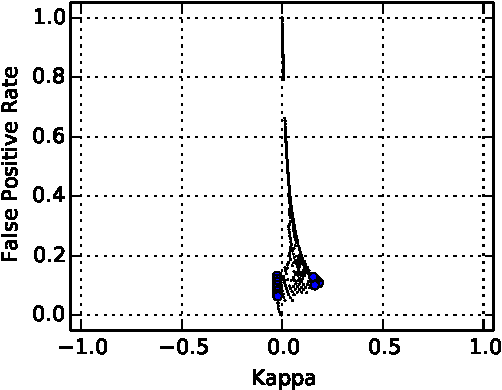
\includegraphics[width=\linewidth]{figs/Kappa-fpr-selected-crop}
        \caption{$\kappa$-$fpr$ diagram}
        \label{fig:MinMax-Kappa-fpr}
    \vspace{0.7cm}
    \end{subfigure}
    \begin{subfigure}[b]{\columnwidth}
        \centering
        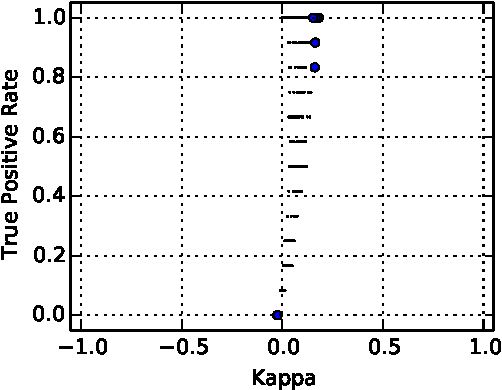
\includegraphics[width=\linewidth]{figs/Kappa-tpr-selected-crop}
        \caption{$\kappa$-$tpr$ diagram}
        \label{fig:MinMax-Kappa-tpr}
    \end{subfigure}
    \caption{Illustration of selected detectors (large blue circles) based on MinMax-Kappa pruning technique. All remaining detectors (small black dots) are pruned.}
    \label{fig:MinMax-Kappa-fpr-tpr}
    \end{adjustbox}
\end{figure}

\begin{figure}[tbh]
    \centering
    \begin{adjustbox}{minipage=\linewidth,scale=0.8}
    \begin{subfigure}[b]{\columnwidth}
        \centering
        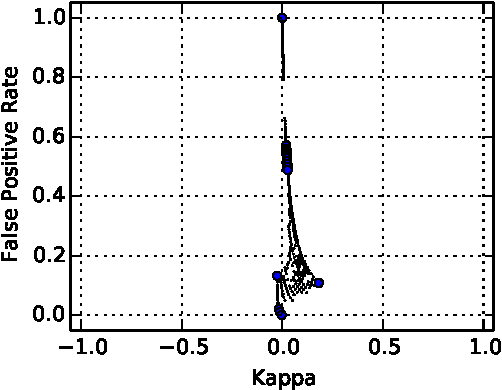
\includegraphics[width=\linewidth]{figs/ROCCH-GT-Kappa-fpr-selected-crop}
        \caption{$\kappa$-$fpr$ diagram}
        \label{fig:ROCCH-Kappa-fpr}
    \vspace{0.7cm}
    \end{subfigure}
    \begin{subfigure}[b]{\columnwidth}
        \centering
        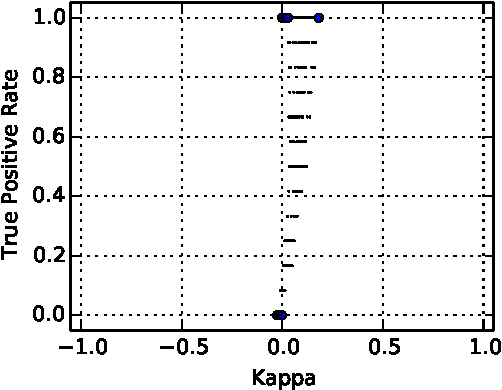
\includegraphics[width=\linewidth]{figs/ROCCH-GT-Kappa-tpr-selected-crop}
        \caption{$\kappa$-$tpr$ diagram}
        \label{fig:ROCCH-Kappa-tpr}
    \end{subfigure}
    \caption{Illustration of selected detectors (large blue circles) based on ROCCH-Kappa pruning technique. All remaining detectors (small black dots) are pruned.}
    \label{fig:ROCCH-Kappa-fpr-tpr}
    \end{adjustbox}
\end{figure}

\begin{figure}[tbh]
    \centering
    \begin{adjustbox}{minipage=\linewidth,scale=0.8}
    \begin{subfigure}[b]{\columnwidth}
        \centering
        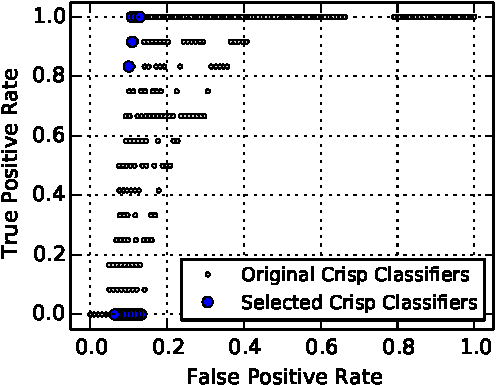
\includegraphics[width=\linewidth]{figs/roc-MinMax-Kappa-selected-crop}
        \caption{MinMax-Kappa pruning}
        \label{fig:ROC-MinMax-Kappa}
    \vspace{0.7cm}
    \end{subfigure}
    \begin{subfigure}[b]{\columnwidth}
        \centering
        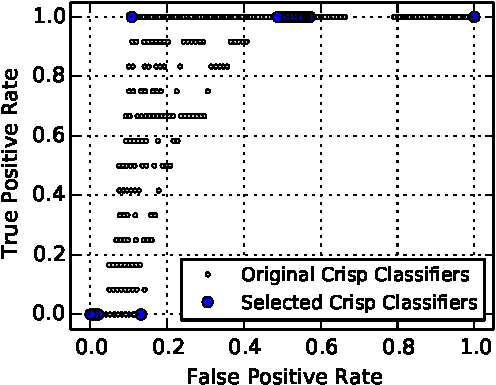
\includegraphics[width=\linewidth]{figs/roc-ROCCH-KAPPA-PairWise-selected-crop}
        \caption{ROCCH-Kappa pruning}
        \label{fig:ROC-ROCCH-Kappa}
    \end{subfigure}
    \caption{Illustration of the selected detectors for combination mapped onto the ROC space (large blue circles). All other detectors (small black dots) can be pruned.}
    \label{fig:ROC-MinMax-vs-ROCCH-Kappa}
    \end{adjustbox}
\end{figure}


\subsection{ROCCH-Kappa Pruning}
\label{sub:rocch-kappa}

This technique also tries to select accurate detectors and then find a set of detectors with complimentary errors.
In contrast with MinMax-Kappa, this technique considers the detectors that are on the facet of the ROCCH in the ROC space.
These detectors are selected since they are the most accurate available detectors that covers the whole range of $fpr$ and $tpr$ trade-off.
The Kappa measure is then used to select diverse detectors with reference to those on ROCCH.
The technique computes the Kappa value of each detector on the ROCCH and all the remaining detectors, sort the resulting values in ascending order.
Detectors with larger values of Kappa are discarded, since they provide similar decisions (or errors) to those provided by the select detectors (on the ROCCH).

The most diverse detectors are those that provide negative or close to zero Kappa values ($\kappa \leq 0$), however are not trivial detectors (providing always either positive or negative decisions).
The only parameter of the ROCCH-Kappa is the number of detectors to be selected for each detector on the ROCCH.
In practice, the number of detectors on the ROCCH is small ([3-20] detectors).
Figure~\ref{fig:ROCCH-Kappa-fpr-tpr} shows an example of the selected detectors from our experiment, according to the ROCCH-Kappa technique, where the Kappa values (on the X-axis) for the selected detectors are plotted against false positive (Figure~\ref{fig:ROCCH-Kappa-fpr}) and true positive  (Figure~\ref{fig:ROCCH-Kappa-tpr}) rates.
Similarly, these selected points (large, blue) are the $\mathcal{C}_{\mbox{selected}}$ in Algorithm~\ref{PBC}, while all remaining detectors (small points) can be pruned.
Figure~\ref{fig:ROC-ROCCH-Kappa} map the detectors selected by ROCCH-Kappa to the ROC space, which could be compared to those selected by MinMax-Kappa in Figure~\ref{fig:ROC-MinMax-Kappa}.

\subsection{MinMax-, ROCCH- Pruning with dCor and dCov}
\label{sub:minmax-rocch-dcov}
These techniques keep using the logic we proposed in section~\ref{sub:minmax-kappa} and section~\ref{sub:rocch-kappa}, the novelty behind them is to use newer and stronger distance correlation, which is described in section~\ref{sec:dcov-dcor}. With the help of these two new metric and integrating them with MinMax and ROCCH technique we can have more confidence in our PBC method that are working well and it is stable all the time and since you use it with a rational measure of agreement you can expect to get the reasonable results.

Here in both dCor and dCov when the result of comparing two different vectors is equal to $0$ it means that they are surely independent of each other; and when the result is equal to $1$ it means they are exactly similar to each other.

\subsection{Expected Value of Boolean Combination}
\label{sub:expected-value}

Expected Value of Boolean Combination (EVBC)
Our other approach for pruning classifiers is using Expected value. To do that we calculate expected values of combinations of each classier with every other classifiers. This is an iterative method that would be applied on every classifier we have. First we select a classifier, classifier X. To calculate expected value of a combination we need to choose another classifier such as classifier Y from our pool of classifiers. Since we have 10 different Boolean operations we could produce 10 different new classifiers by combining classifier X and Y. Here, we explain our formula for one of the Boolean operation but we could easily extend it for all the rest.

As we explained earlier we could identify each classifier by its TPR-FPR on ROC curve, therefore we want to calculate expected value of TPR-FPR of the new classifier. To calculate TPR and FPR of the combination ($tpr_C, fpr_C$) from Classifier X with ($TPR_X, FPR_X$) and classifier $Y$ with ($TPR_Y, FPR_Y$) we use the equations below:

\begin{multline}
% \begin{equation}
TPR_C = B1 \times TPR_X \times TPR_Y+B2\times TPR_X \times(1- TPR_Y)+\\B3\times(1- TPR_X)\times TPR_Y+B4\times(1- TPR_X)\times(1- TPR_Y)
% \end{equation}
\end{multline}

\begin{multline}
% \begin{equation}
FPR_C = B1 \times FPR_X \times FPR_Y+B2\times FPR_X \times(1- FPR_Y)+\\B3\times(1-FPR_X)\times FPR_Y+B4\times(1- FPR_X)\times(1-FPR_Y))
% \end{equation}
\end{multline}


Which B1, B2, B3, B4 is binary representation of our Boolean operation (And = '1000', OR = '1110', XOR = '0110', etc. )
For example for XOR we would have:

\begin{multline}
% \begin{equation}
TPR_C = 0 \times TPR_X \times TPR_Y+1\times TPR_X \times(1- TPR_Y)+\\1\times(1- TPR_X)\times TPR_Y+0\times(1- TPR_X)\times(1- TPR_Y)
% \end{equation}
\end{multline}

\begin{multline}
% \begin{equation}
FPR_C = 0 \times FPR_X \times FPR_Y+1\times FPR_X \times(1- FPR_Y)+\\1\times(1-FPR_X)\times FPR_Y+0\times(1- FPR_X)\times(1-FPR_Y))
% \end{equation}
\end{multline}

Now we have 3 classifiers X, Y and the combination of them using XOR operation (Classifier C) as it's shown in the picture below. Now we need to evaluate the goodness of classifier C compared to X and Y. Area Under the Curve (AUC) is a function, which can be used to evaluate the goodness. Based on the coordination of each classifier on ROC curve we can compute AUC of the classifier with the following formula:


\begin{figure}[H]
\centering
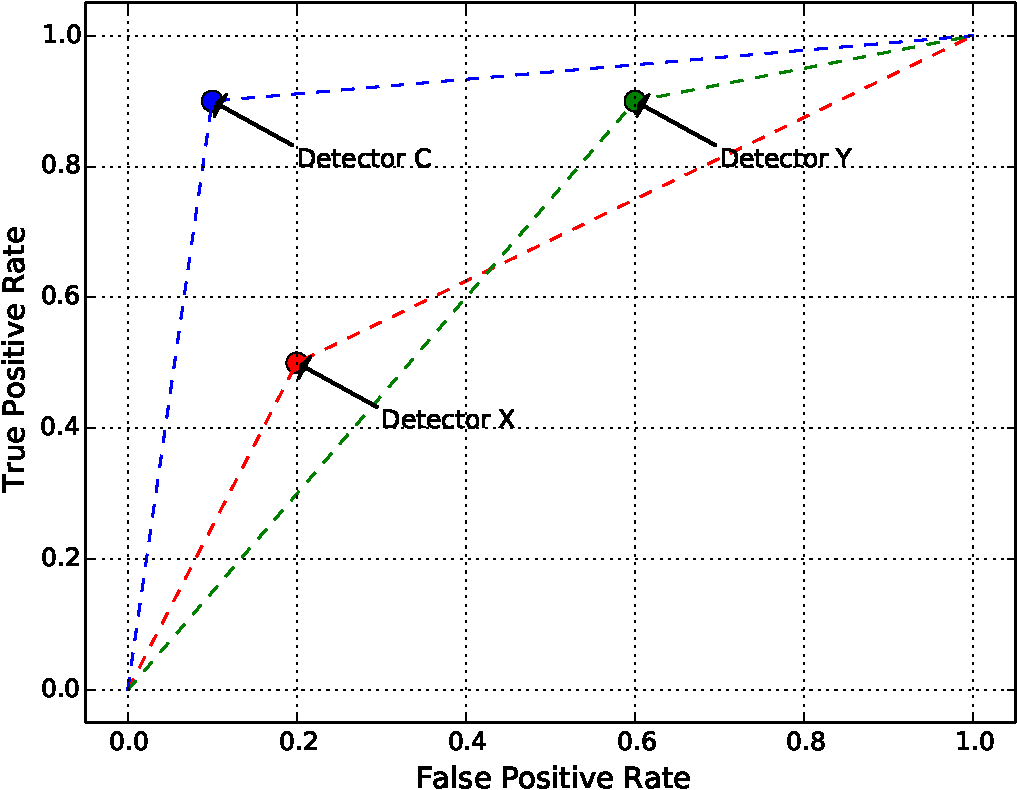
\includegraphics[scale=0.75]{figs/Classifiers_X_Y_C}
\caption{Combination of classifier X and Y lead to C}
\label{fig::X_Y_C}
\end{figure}


We compute AUC for classifier X, Y and C and keep classifier C only if its AUC is greater than AUC of both classifiers X and Y. Greater AUC means that our classifier is much closer to the ground truth (which will give us the TPR = 1 and FPR = 0).
If AUC$_C$ is greater than AUC$_X$ and AUC$_Y$ we keep the difference in AUC as the improvement of that classifier with the specific Boolean operation used. The variable that keeps the improvement for classifier X is IMP as defined below:
$IMP_X  = AUC_C - Max(AUC_X, AUC_Y)$
We calculate $IMP_X$ for all 10 Boolean operations and add them to the previous value. At the end, $IMP_X$ has the expected value of all of the combination possible between classifiers X and Y using 10 Boolean operations. We repeat these steps for classifier X in combination with the rest of classifiers, choosing one each time as a new classifier Y and update $IMP_X$. The final $IMP_X$ value has the total expected value of the improvement with respect to all the combinations if we select classifier X. After we compute $IMP_X$ for classifier X and the rest of classifiers we will update the value in our table in a $TPR_X$ $FPR_X$ position with $IMP_X$. We repeat all these steps for every classifier we have and update their IMP in the table and then we can create a table shown below with each cell representing the expected value of the classifier combinations getting improved. We select that classifier with the most improvement.

\begin{figure}[H]
\centering
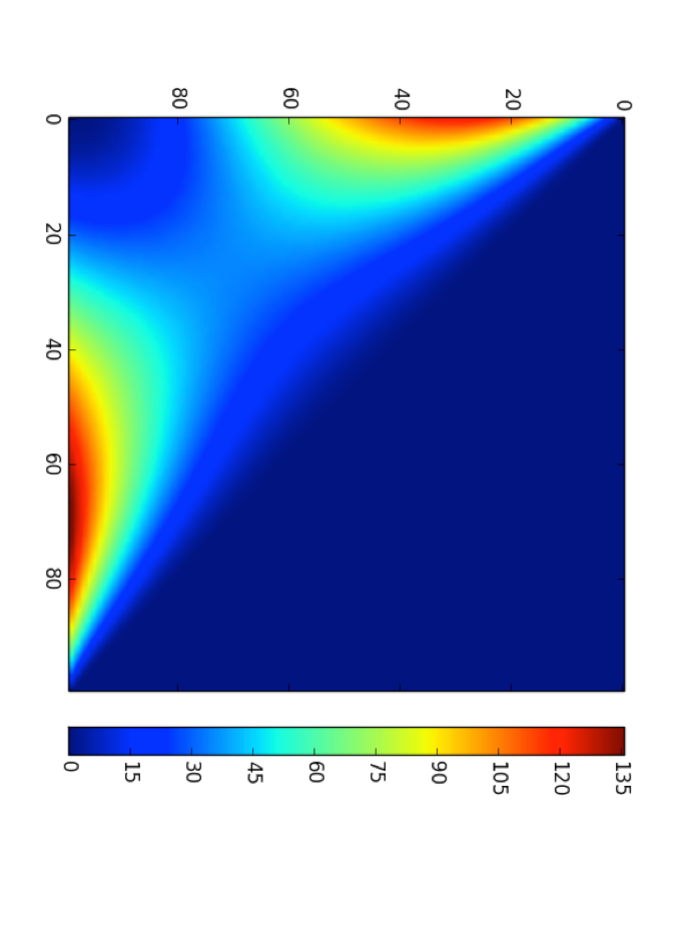
\includegraphics[scale=1]{figs/expected_value}
\caption{expected value of all classifiers in the ROC space}
\label{fig::expected_value}
\end{figure}

As shown in Figure~\ref{fig::expected_value}  the representation of that table if we use color plotting. The red region shows classifiers with higher IMP and the blue region shows classifier with low IMP. That means if we select our basket of classifiers from red region we would have a higher chance to get better classifiers after combination of those pruned classifiers. Our assumption for creating above table was that we have all the possible classifiers with 2 digits precision and after computing all possible combination for all the classifiers we set the value of each cell below minor diameter to zero (all the classifiers below random line) since want to evaluate goodness of classifiers better than random guess.
We can re-produce the same table by computing the expected value of combination just for the classifiers that already we have; by doing that we will get the below table (plot) and we can prune our classifier based on this new table.

\section{Complexity Analysis}
\label{sub:complexity}

Given $K$ soft detectors, let $n_i$ be the number of decision thresholds or crisp detectors produced by each of the soft detector $D_i$, $i=1,\ldots, K$, on the validation set $\mathcal{V}$.
Let $n=\sum_{i=1}^{K} n_i$ the total number of crisp detectors in the ensembles, and $n_{avg} = n/K$ the average number of crisp detectors produced by soft detectors.

A brute-force search for optimal combination is infeasible in practice due to the doubly exponential combinations.
In fact, for $n$ crisp detectors there are $2^n$ possible outcomes that can be combined in $2^{2^n}$ ways, which makes the brute-force combination impractical even for small $n$ values \cite{Barreno2008}.
Even only pairwise combination of $n$ crisp detectors, which requires $\mathcal{O}(n^2)$ Boolean operations, may not be feasible in practise for large $n$ values.
The sequential combination of the IBC algorithm reduces its worst-case time complexity to $\mathcal{O}(n_{avg}^2 + Kn_{avg})$ Boolean operations.

Both pruning techniques are capable of reducing the size of the selected subset of detectors (for Boolean combination) up to a user defined maximum number ($U$).
The worst-case time complexity required by MinMax-Kappa technique to select $U$ crisp detectors (and prune the rest) is $\mathcal{O}(n(\log n + 1) + U^2)$.
It requires about $n(\log n + 1)$ operations for computing and sorting the Kappa values for all crisp detectors, and $U^2$ for the pairwise Boolean combinations of the $U$ retained detectors.
For ROCCH-Kappa technique however the worst-case time complexity is of the order $\mathcal{O}(n(\log n +n_{ev}) + U^2)$, where $n_{ev}$ is the number of emerging vertices which is typically around ten.
The additional $n_{ev}$ factor is due to the computation of Kappa is repeated $n_{ev}$ times for each emerging point on the ROCCH.
For numerical comparison, Table~\ref{tab:time-complexity} shows the average time for each combination and pruning technique used in our experiments.

